%%%%%%%%%%%%%%%%%%%%%%%%%%%%%%%%%%%%%%%%%
% University/School Laboratory Report
% LaTeX Template
% Version 4.0 (March 21, 2022)
%
% This template originates from:
% https://www.LaTeXTemplates.com
%
% Authors:
% Vel (vel@latextemplates.com)
% Linux and Unix Users Group at Virginia Tech Wiki
%
% License:
% CC BY-NC-SA 4.0 (https://creativecommons.org/licenses/by-nc-sa/4.0/)
%
% Modifications made:
% 1. Replaced title, name, date, date performed, and instructor with personal details
% 2. Removed partners row
% 3. Replaced original structure with personal structure
% 
%%%%%%%%%%%%%%%%%%%%%%%%%%%%%%%%%%%%%%%%%

%----------------------------------------------------------------------------------------
%	PACKAGES AND DOCUMENT CONFIGURATIONS
%----------------------------------------------------------------------------------------

\documentclass[
	letterpaper, % Paper size, specify a4paper (A4) or letterpaper (US letter)
	12pt, % Default font size, specify 10pt, 11pt or 12pt
]{CSUniSchoolLabReport}

\nocite{*}
\addbibresource{bibliography.bib} % Bibliography file (located in the same folder as the template)

%----------------------------------------------------------------------------------------
%	REPORT INFORMATION
%----------------------------------------------------------------------------------------

\title{Determination of the \\ Molar Enthalpy of Combustion of Paraffin Wax \\ IB Chemistry HL} % Report title

\author{Ethan \textsc{Chen}} % Author name(s), add additional authors like: '\& James \textsc{Smith}'

\date{September 29, 2023} % Date of the report

%----------------------------------------------------------------------------------------

\begin{document}

\maketitle % Insert the title, author and date using the information specified above

\begin{center}
  \begin{tabular}{l r}
    Date Performed: & September 18, 2023 \\ % Date the experiment was performed
    Instructor:     & Mr \textsc{Deis}   % Instructor/supervisor
  \end{tabular}
\end{center}

% If you need to include an abstract, uncomment the lines below
%\begin{abstract}
%	Abstract text
%\end{abstract}

%----------------------------------------------------------------------------------------
%	OBJECTIVE
%----------------------------------------------------------------------------------------

\section{Purpose}

The purpose of this lab was to determine the molar enthalpy of the combustion of Paraffin Wax (\ce{C25H52(s)}) in the following reaction:

\begin{center}
  \ce{C25H52(s) + 38O2(g) -> 25CO2(g) + 26H2O(g)}
\end{center}


\section{Evidence}

\subsection{Qualitative Observations}

% Paraffin Wax
The Paraffin Wax candle appears white and opaque, with the colour fading into orange nearing the bottom.
Upon touch, the Paraffin Wax feels slightly slippery, and after putting the candle down, the slippery sensation
transfers to your hands.
\\
The Paraffin Wax candle was able to be attached to the watchglass by exposing the
bottom of the candle to a flame, in which the melted paraffin wax at the bottom
was able to stick onto the watchglass. This indicates that melted paraffin wax exhibits
adhesive properties.
\\
The container surrounding the base of the Paraffin Wax candle does not leave
any openings for air to escape other than the opening at the top.
\\
These observations are shown in Figure \ref*{fig:paraffin}.

\begin{figure}[H] % [H] forces the figure to be placed exactly where it appears in the text
  \centering % Horizontally center the figure
  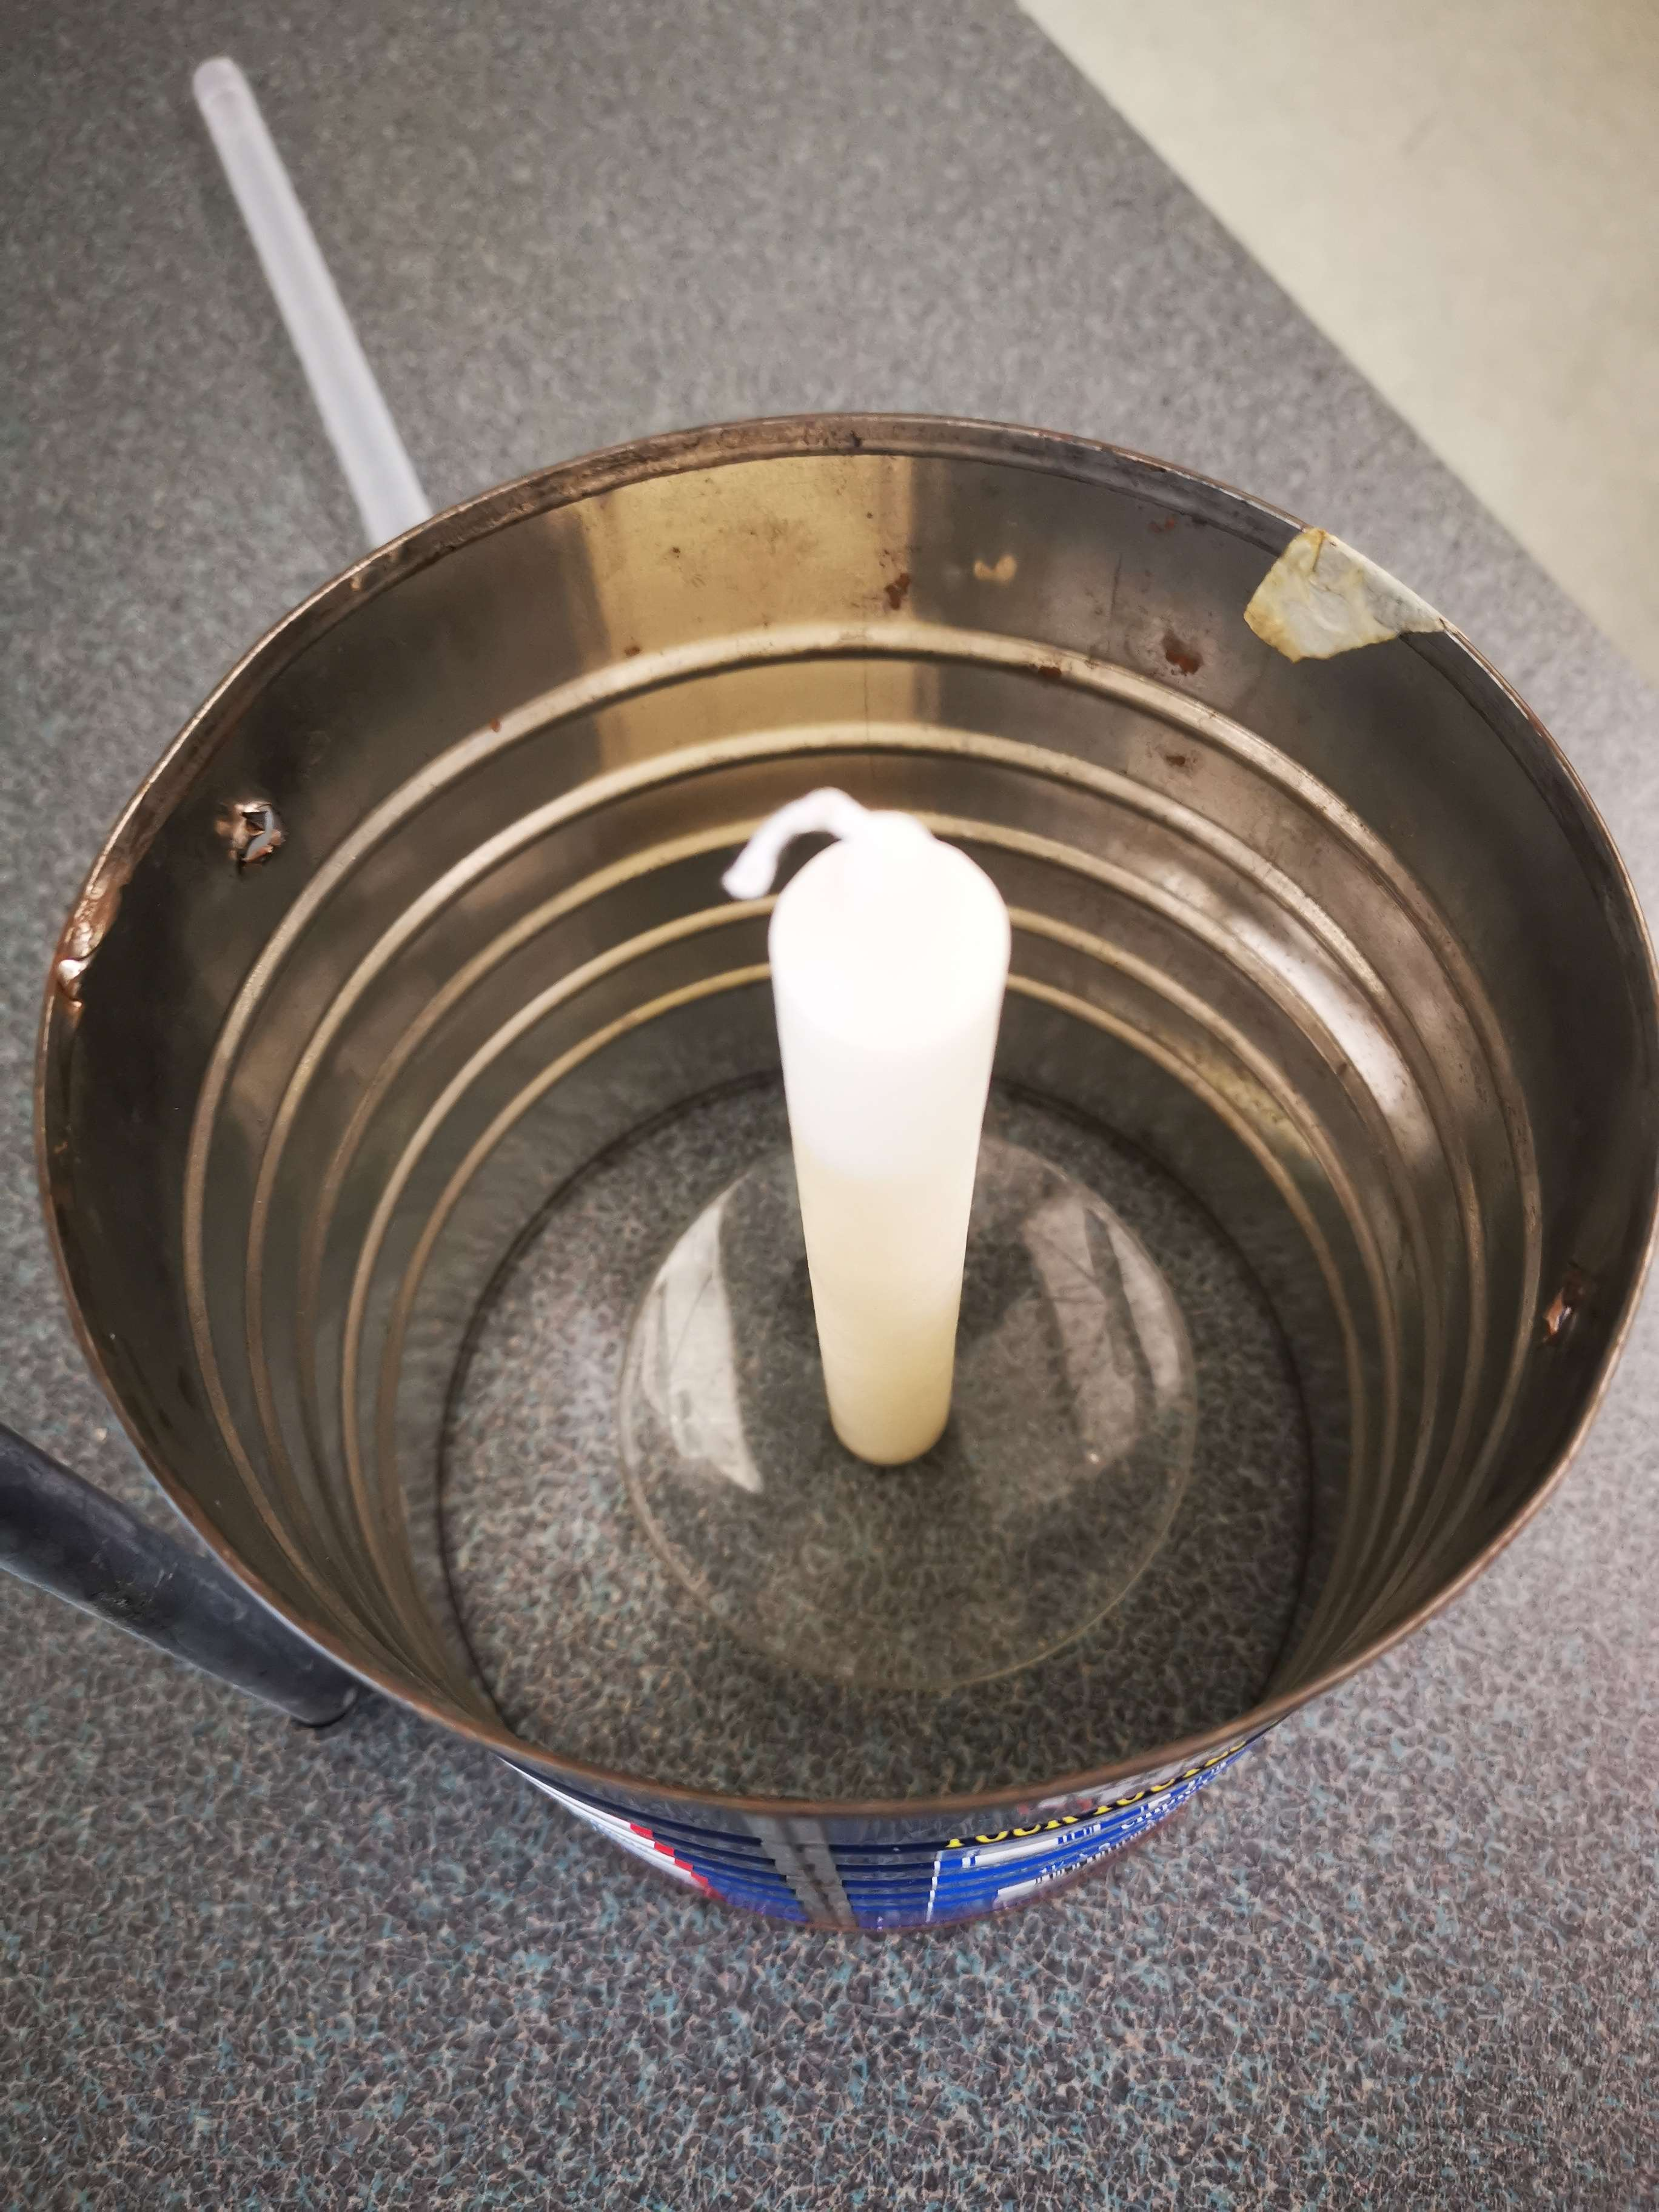
\includegraphics[width=0.65\textwidth]{Paraffin Wax} % Include the figure
  \caption{Appearance of the Paraffin Wax candle attached to watchglass within container.}
  \label{fig:paraffin}
\end{figure}

% Can holding water Top View
The can containing the water has a proportionally greater height than diameter.
The opening at the top of the can is significantly wider than the diameter of the thermometer,
indicating that the space within the can is not entirely closed and isolated.
The two holes allowing for the rod to pass through does wrap around the rod
tightly, however because it is a manually created hole, it still allows for passage
of air within the can and outside the can. These observations are shown in
Figure \ref*{fig:cantop}.
\begin{figure}[H]
  \centering
  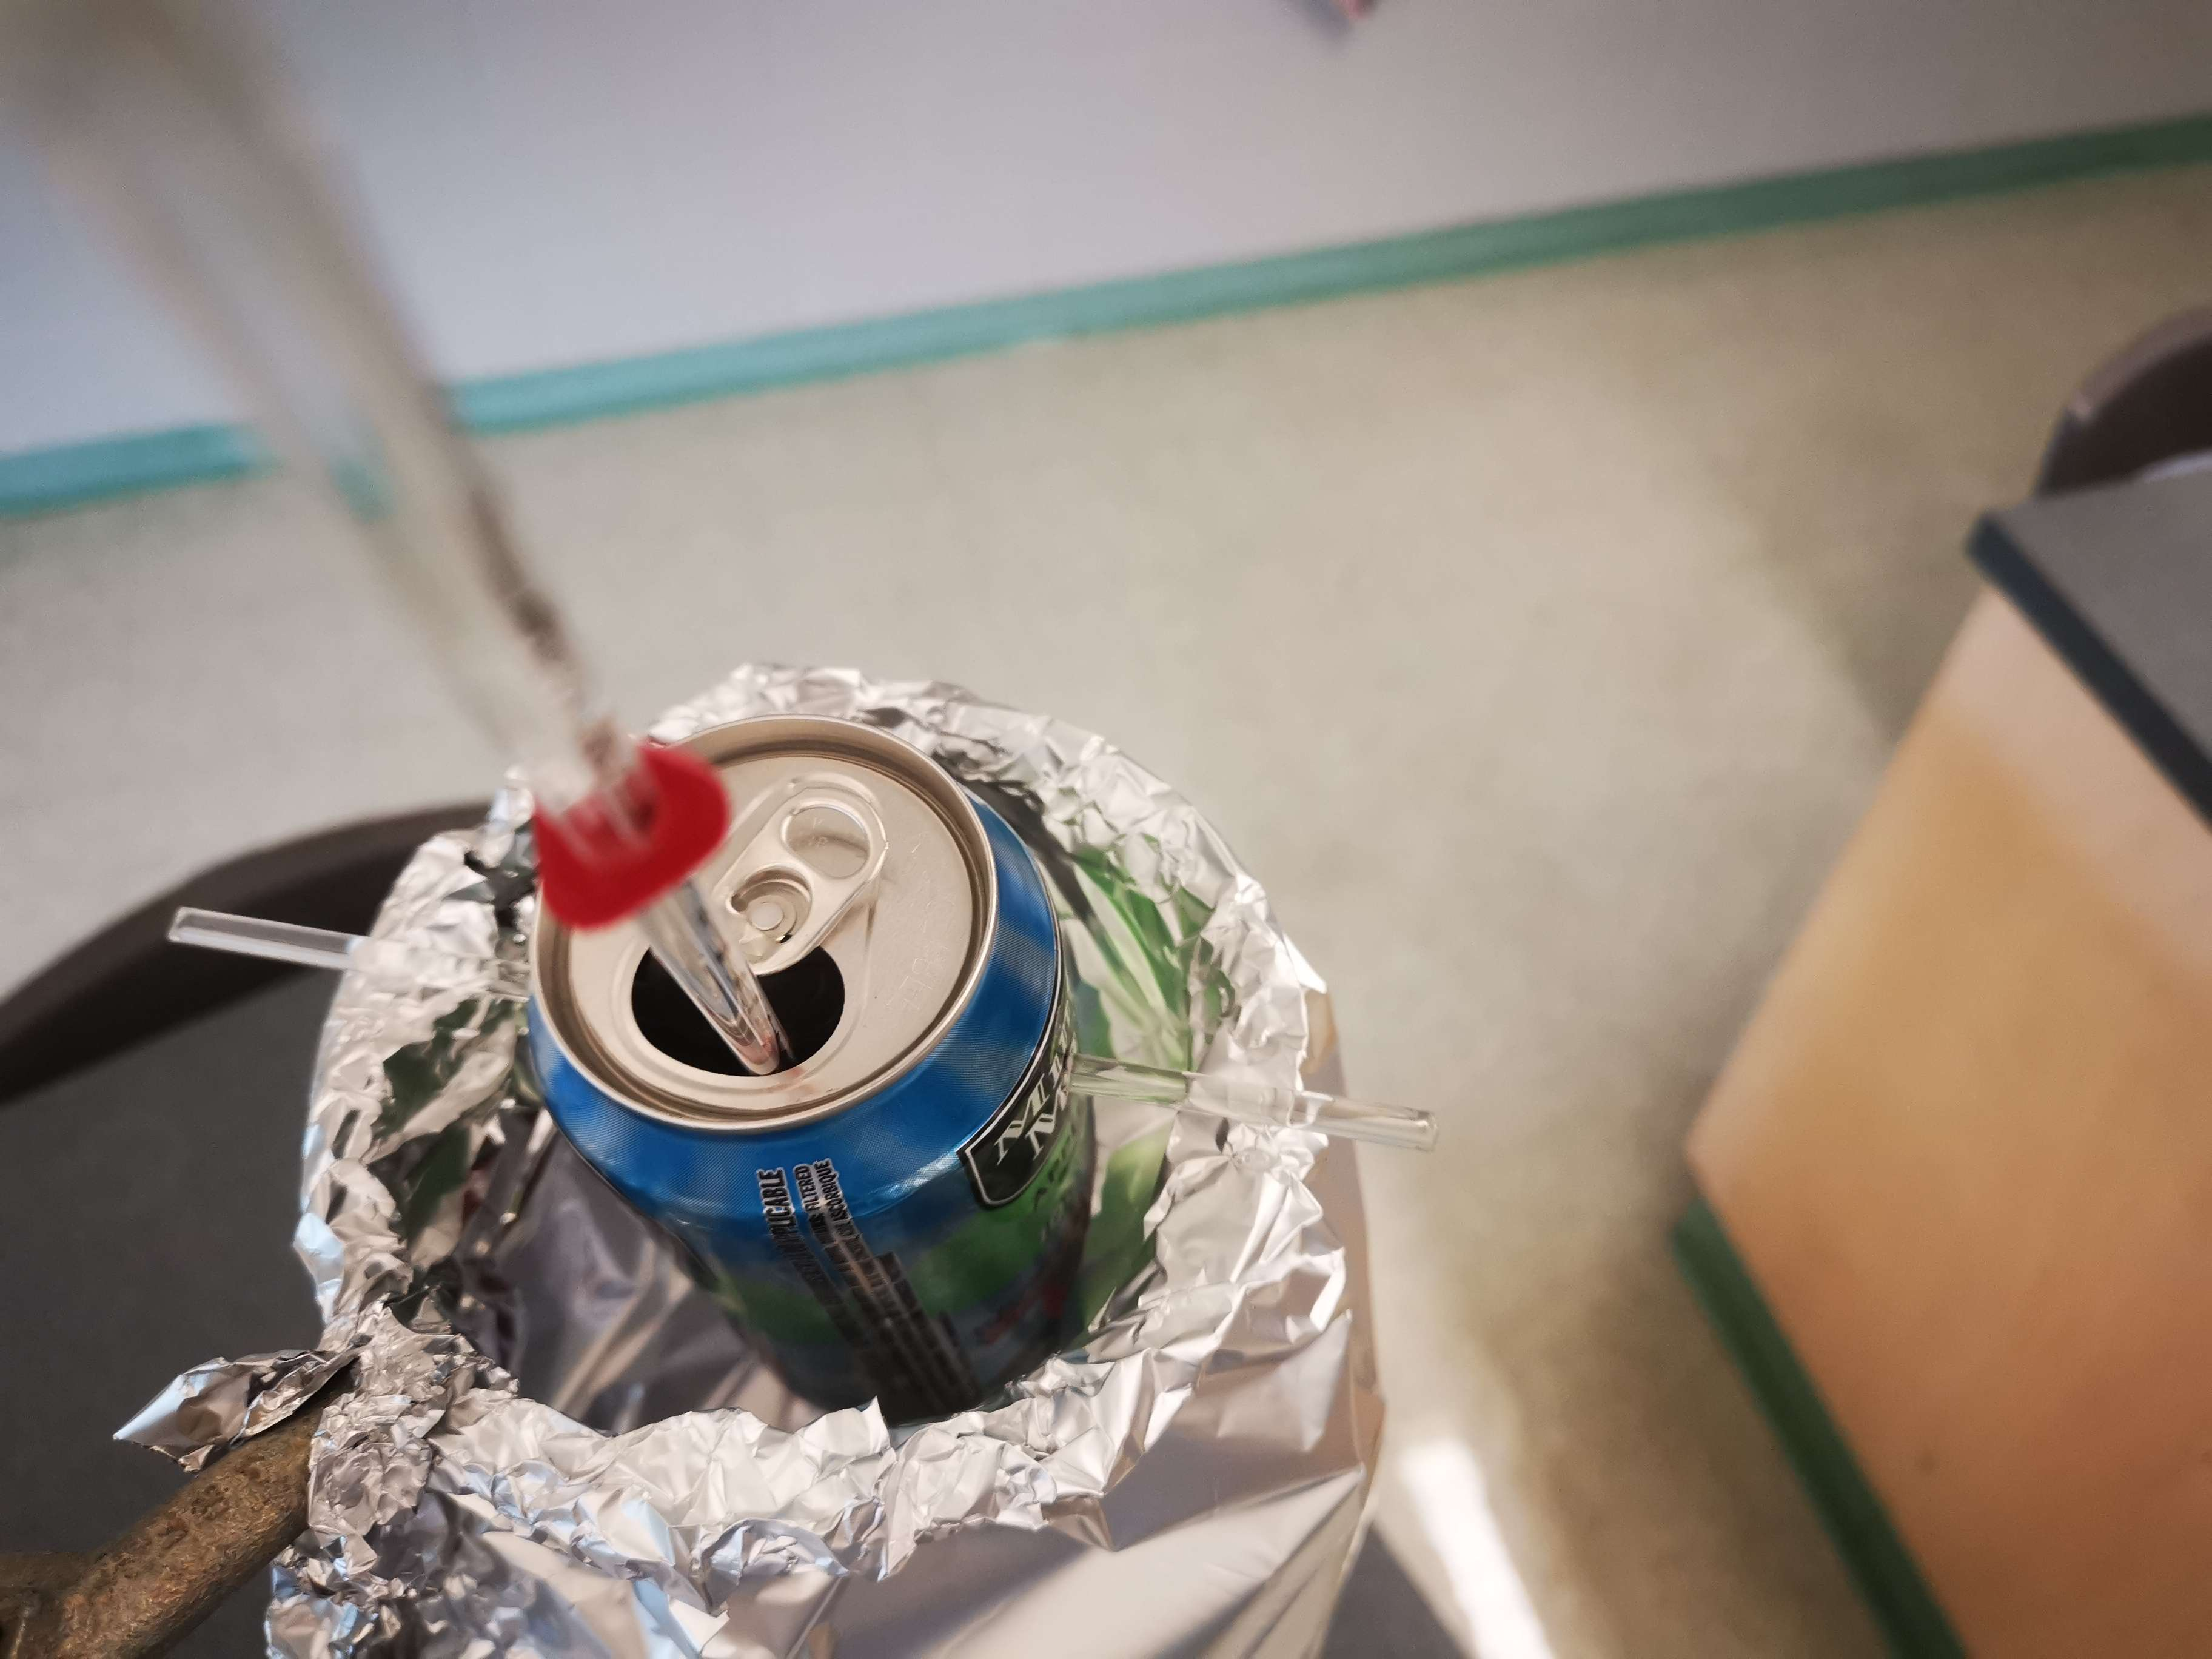
\includegraphics[width=0.65\textwidth]{top}
  \caption{Appearance of can used to contain the water from a top view}
  \label{fig:cantop}
\end{figure}

%Aluminium Foil
The Aluminium Foil surrounding the can leaves an opening at the top between
the ring and the diameter of the can, as seen in Figure \ref*{fig:cantop}.
\\
The process of conducting a trial involved raising the ring along the Ring Stand,
lighting the candle, and lowering the ring. This means that there is an interval of time
from lighting the candle where combustion was not taking place within the calorimeter.
Additionally, after lowering the ring to a reasonable height where the bottom of the
aluminium foil surrounding the can meets the top of the container surrounding the
candle, the two ends of the aluminium foil become separated due to the significantly
larger diameter of the container at the bottom. This leaves a few openings at the side
of the aluminium foil cylinder.
\\
Some of these observations can be seen in Figure \ref*{fig:canside}.
\begin{figure}[H]
  \centering
  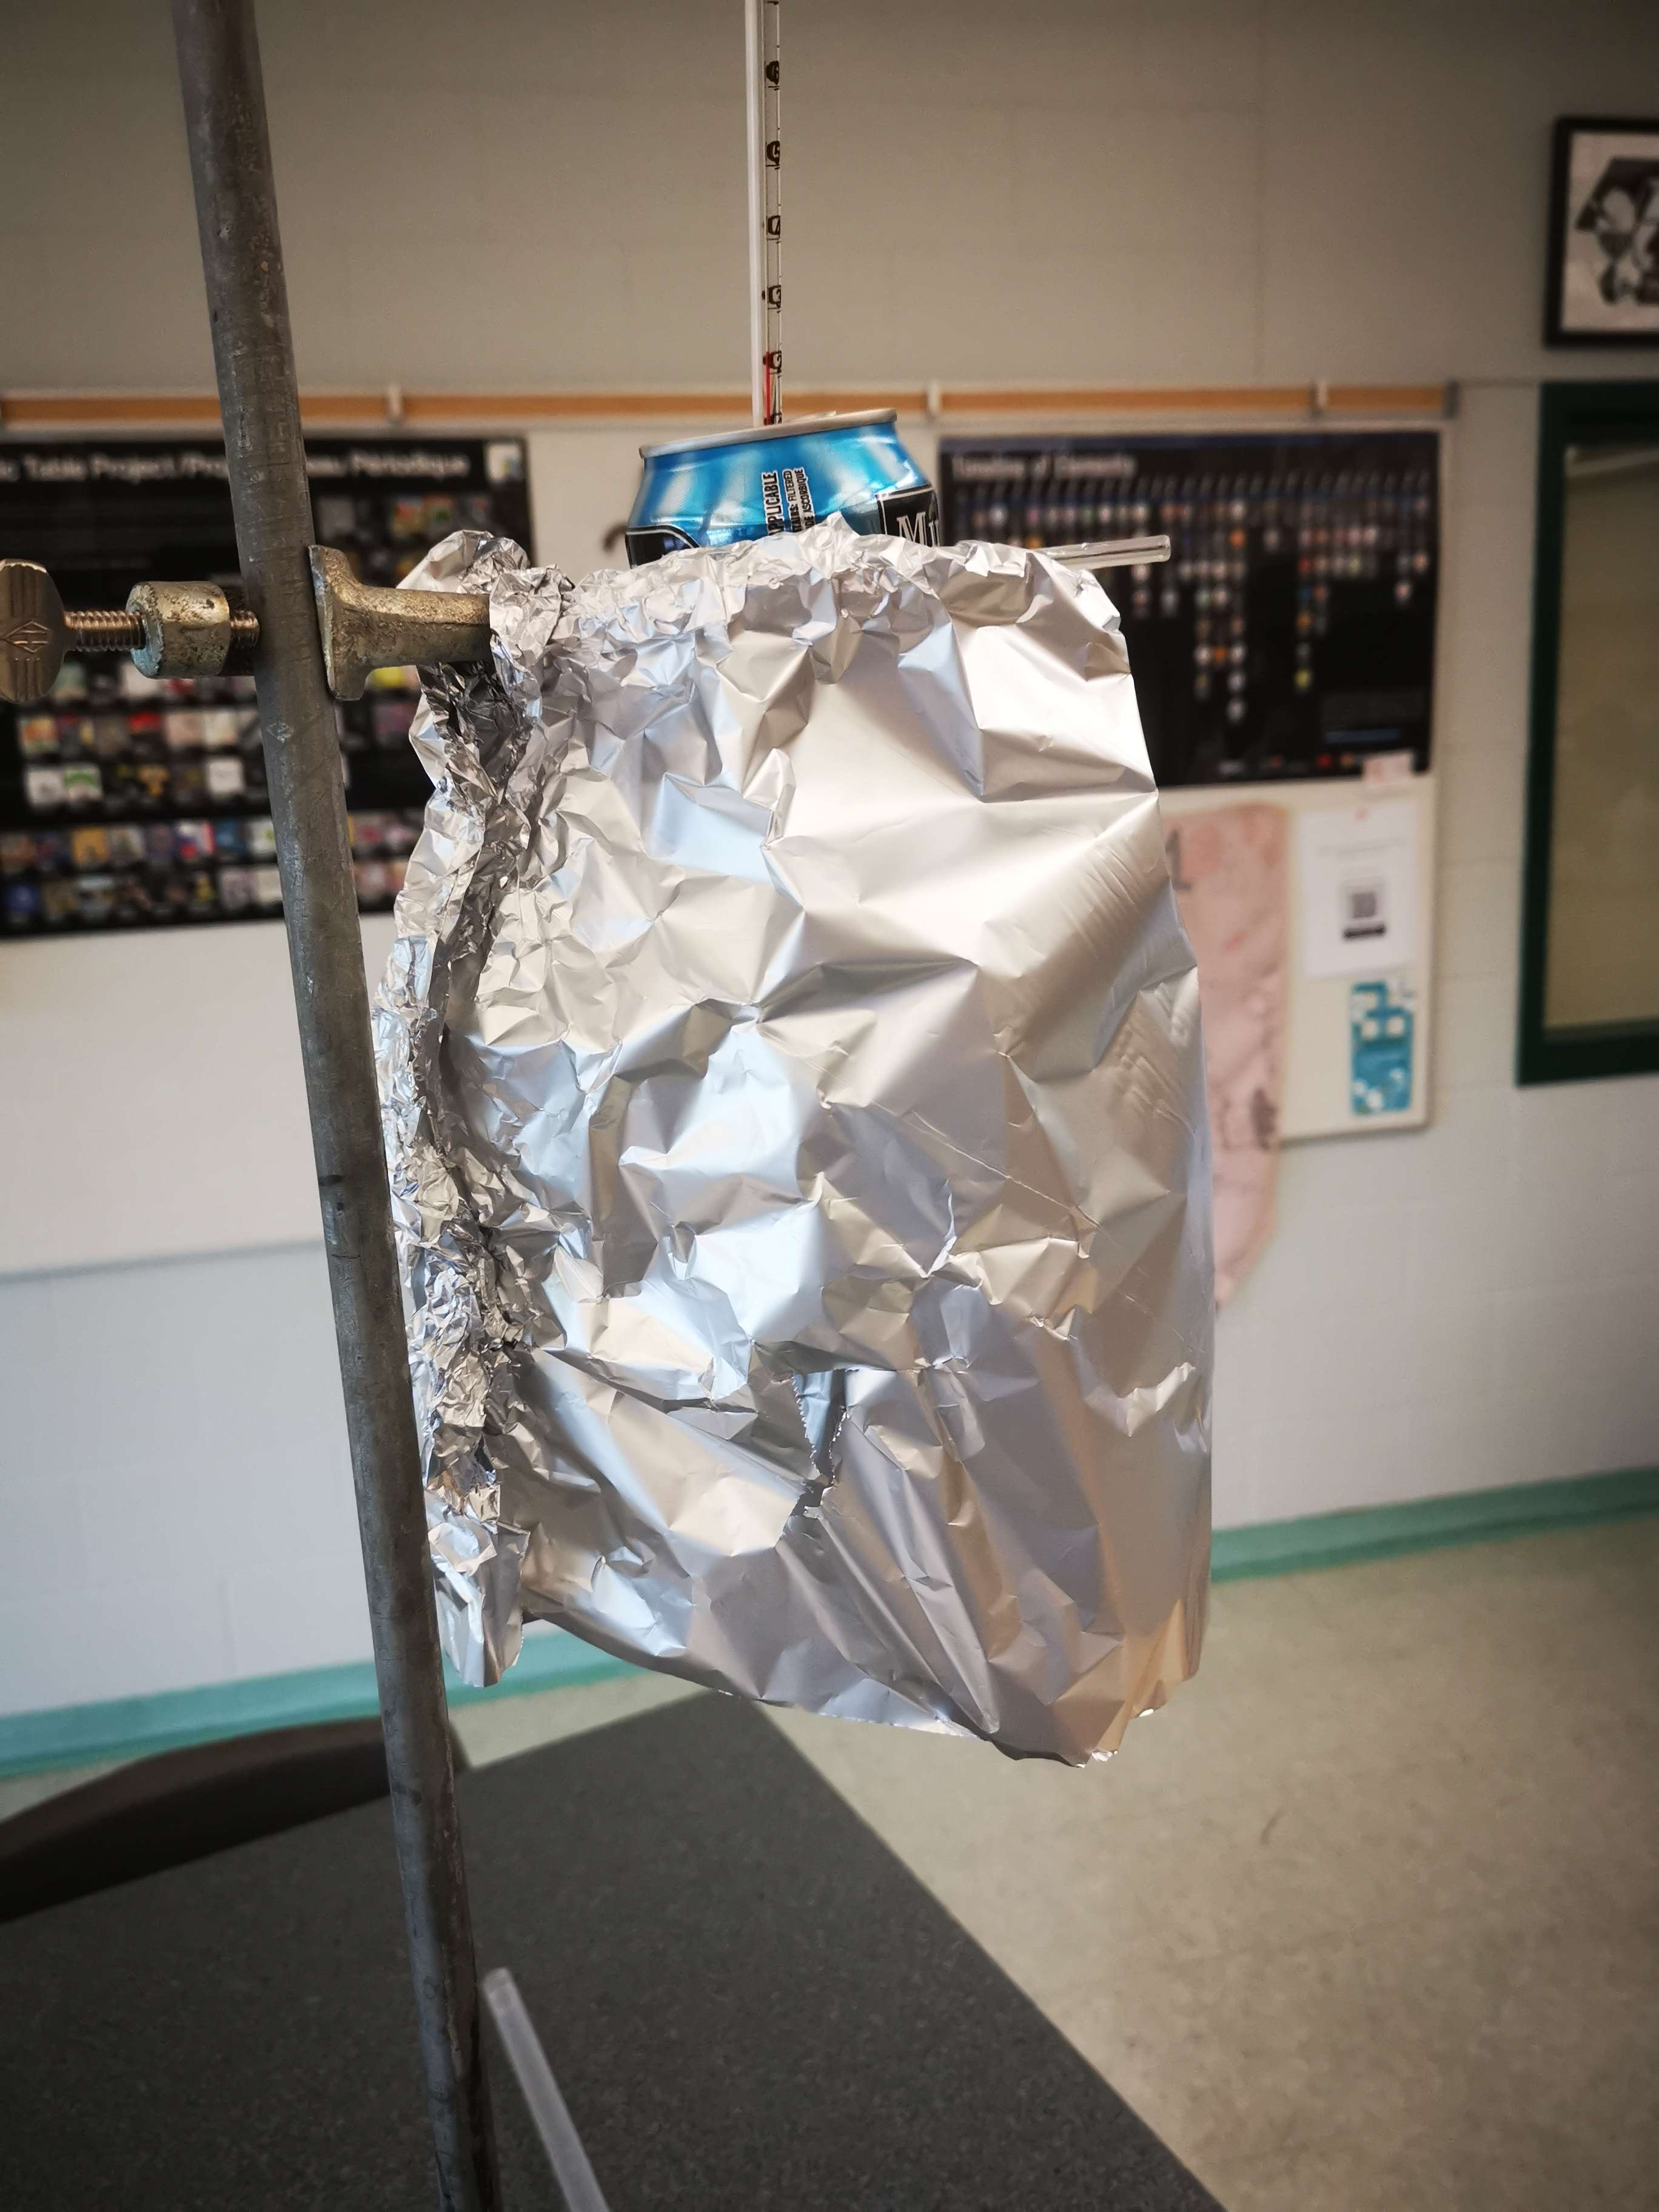
\includegraphics[width=0.65\textwidth]{side}
  \caption{View of aluminium foil attached around elevated ring on ring stand}
  \label{fig:canside}
\end{figure}

%Can bottom
As seen in Figure \ref*{fig:canbottom}, there is a black stain on the bottom of the can
containing the bottom. This is presumably solid carbon produced by incomplete combustion
from previous calorimetry experiments.
\begin{figure}[H]
  \centering
  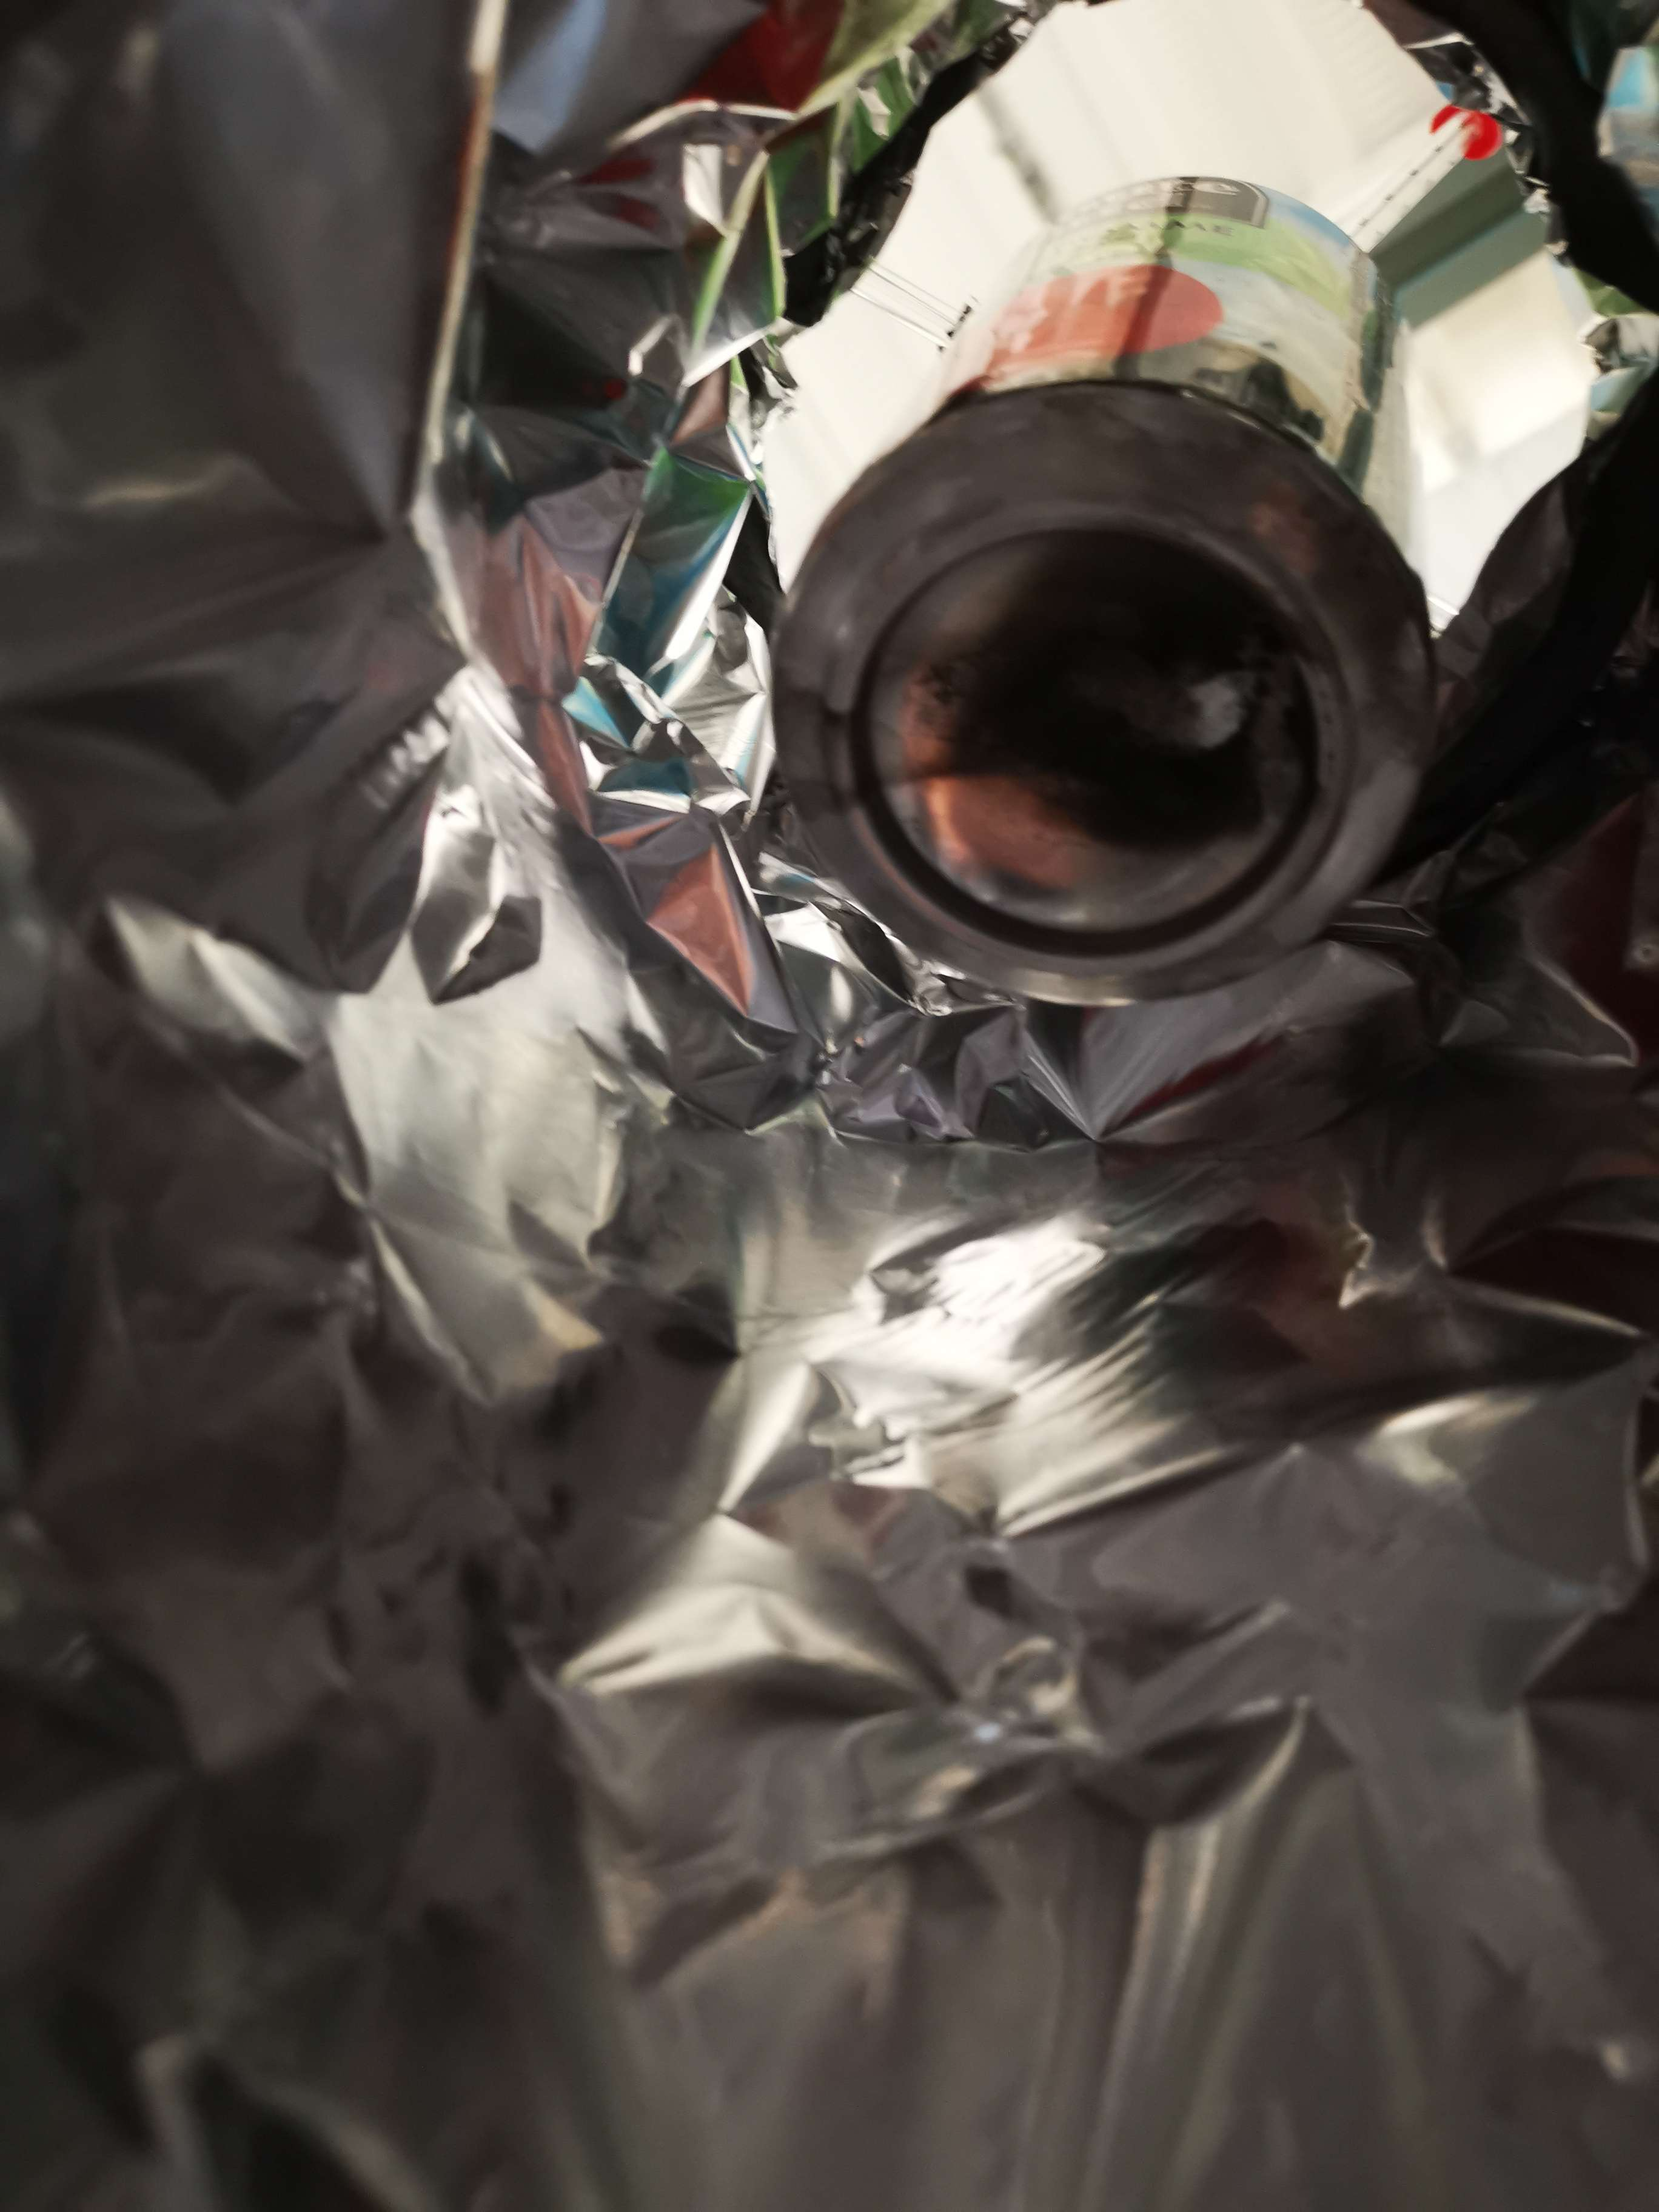
\includegraphics[width=0.65\textwidth]{bottom}
  \caption{Appearance of black stain on the bottom of the can containing water}
  \label{fig:canbottom}
\end{figure}

\subsection{Quantitative Data}

The raw data recorded from the experiment is recorded in Table \ref*{tab:rawdata}.
Note that when measuring the mass of the water, the lab scale was tared
with the can, then water was added into the can. Therefore, the mass recorded
doesn't need to be subtracted by the mass of the can.

\begin{table}[H]
  \centering
  \resizebox{\linewidth}{!}{%
    \begin{tblr}{
      width = \linewidth,
      colspec = {|Q[406]|Q[169]|Q[169]|Q[169]|},
      }
      \hline
      Trial Number & 1 & 2 & 3 \\
      \hline
      {Mass of can /g          \\(±0.003g)} & 13.039 & 15.769 & 15.080\\
      \hline
      {Mass of water /g        \\(±0.003g)} & 50.141 & 50.112 & 50.105\\
      \hline
      {Initial mass of candle  \\and watch glass /g\\(±0.003g)} & 106.907 & 106.209 & 105.691\\
      \hline
      {Final mass of candle    \\and watch glass /g\\(±0.003g)} & 106.209 & 105.691 & 105.240\\
      \hline
      {Initial Temperature     \\of water /\textcolor[rgb]{0.302,0.318,0.337}{°}C\\(±0.3~\textcolor[rgb]{0.302,0.318,0.337}{°}C)} & 23.8 & 25.0 & 25.0\\
      \hline
      {Final Temperature       \\of water /\textcolor[rgb]{0.302,0.318,0.337}{°}C\\(±0.3~\textcolor[rgb]{0.302,0.318,0.337}{°C})} & 60.7 & 51.2 & 52.6\\
      \hline
    \end{tblr}
  }
  \caption{Raw data recorded from each trial during the experiment}
  \label{tab:rawdata}
\end{table}


Something else to keep in mind is that the final temperature of the water was determined by
setting a timer for 5 minutes and recording the temperature afterwards. However,
for the first trial, we forgot to consider after what period of time would we record
the final temperature. Therefore, that trial simply involved noting the temperature after twenty
15 second intervals which was manually counted. This demonstrates a reason why
the final temperature of the water for the first trial was significantly different than
the two other trials.

\section{Analysis}

\subsection{Calculation of theoretical molar enthalpy\\ of combustion}

The theoretical molar enthalpy of combustion for Paraffin Wax \\(\ce{C25H52(s)}) will be
calculated using Hess' Law.

With \(\Delta H\degree_{f}\) being the molar enthalpy of formation for some compound,
the following values will be used.
\\
\begin{tabular}{ll}
  \ce{C25H52(s)}: & \(\Delta H\degree_{f} = -1424.3~kJmol^{-1}\) \\
  \ce{CO2(g)}:    & \(\Delta H\degree_{f} = -393.5~kJmol^{-1}\)  \\
  \ce{H2O(g)}:    & \(\Delta H\degree_{f} = -241.8~kJmol^{-1}\)
\end{tabular}

These values can then be used to calculated to theoretical molar enthalpy of combustion for Paraffin Wax.

\begin{align*}
  let~\Delta H\degree_{comb} & = \mbox{the molar enthalpy of combustion for Paraffin Wax } /kJ      \\
  let~n                      & = \mbox{the amount of a compound } /mol                              \\
  let~\Delta H\degree_{f}    & = \mbox{the molar enthalpy of formation for a compound } /kJmol^{-1} \\
\end{align*}

\begin{multline*}
  \Delta H\degree_{comb} = \Sigma nH\degree_{f}products - \Sigma nH\degree_{f}reactants \\
  \Delta H\degree_{comb} = \left((25mol)(-393.5kJmol^{-1}) + (26mol)(-241.8kJmol^{-1})\right)\\ - (1mol)(-1424.3kJmol^{-1})
\end{multline*}
\[\Delta H\degree_{comb} = -14700kJ\]
\[\Delta H\degree_{comb} = -14.7MJ\]

\subsection{Calculation of experimental molar enthalpy\\ of combustion}
The system of the calorimetry experiment will be the combustion of the Paraffin Wax,
and the surroundings will be the water and the can. We will make the assumption that
the can is made out of aluminium (\cite{Drink_can_2023}).

The systems and surroundings are presented in Table \ref*{tab:system} along with
what they entail. Note that \(q\) equals to the total heat in J.

\begin{table}[H]
  \centering
  \resizebox{\linewidth}{!}{%
    \begin{tabular}{>{\hspace{0pt}}m{0.369\linewidth}|>{\hspace{0pt}}m{0.569\linewidth}}
      System                                                                       & Surroundings                                                                                                                     \\
      \hline
      Combustion of Paraffin Wax\par{}\(\Delta E_p\)\par{}\(q_1=nH\degree_{comb}\) & Water + Aluminium Can\par{}\(\Delta E_k\)\par{}\(q_2=m_{water}c_{water}\Delta T_{water}\)\par{}\(q_3=m_{Al}c_{Al}\Delta T_{Al}\)
    \end{tabular}
  }
  \caption{System and surroundings of the calorimeter.}
  \label{tab:system}
\end{table}

Given that \(q_1=q_2+q_3\), the value of \(nH\degree_{comb}\) can then be calculated. A sample calculation is shown below for Trial 1.
\begin{align*}
  q_1              & = q_2 + q_3                                                                \\
  nH\degree_{comb} & = m_{water}c_{water}\Delta T_{water} + m_{Al}c_{Al}\Delta T_{Al}           \\
  H\degree_{comb}  & = \frac{m_{water}c_{water}\Delta T_{water} + m_{Al}c_{Al}\Delta T_{Al}}{n} \\
\end{align*}
\begin{multline*}
  m_{water}c_{water}\Delta T_{water} + m_{Al}c_{Al}\Delta T_{Al} \\ = (50.141g \pm 0.003g)(4.19Jg^{-1}\degree C^{-1})(60.7\degree C \pm 0.3\degree C - 23.8\degree C \pm 0.3\degree C) \\+ (13.039g \pm 0.003g)(0.897Jg^{-1}\degree C^{-1})(60.7\degree C \pm 0.3\degree C - 23.8\degree C \pm 0.3\degree C)
\end{multline*}
\begin{multline*}
  m_{water}c_{water}\Delta T_{water} + m_{Al}c_{Al}\Delta T_{Al} \\ = (50.141g \pm 0.006\%)(4.19Jg^{-1}\degree C^{-1})(36.9\degree C \pm 2\%) \\ + (13.039g \pm 0.02\%)(0.897Jg^{-1}\degree C^{-1})(36.9\degree C \pm 2\%)
\end{multline*}
$m_{water}c_{water}\Delta T_{water} + m_{Al}c_{Al}\Delta T_{Al} = 8.18 \times 10^3J \pm 4\%$

\begin{align*}
  n & = (106.907 \pm 0.003g - 106.209g \pm 0.003g)(\frac{1mol}{352.77g})
  \\
  n & = (0.698g \pm 0.9\%)(\frac{1mol}{352.77g})
  \\
  n & = 1.98 \times 10^{-3} mol \pm 0.9\%
\end{align*}

\begin{align*}
  H\degree_{comb} & = \frac{8.18 \times 10^3J \pm 4\%}{1.98 \times 10^{-3} mol \pm 0.9\%}
  \\
  H\degree_{comb} & = -4.1MJmol^{-1} \pm 0.2 MJmol^{-1}
\end{align*}

Table \ref*{tab:experCalc} presents the calculated experimental molar enthalpies of combustion for each trial.

\begin{table}[H]
  \centering
  \begin{tabular}{|l|l|}
    \hline
    Trial Number & \begin{tabular}[c]{@{}l@{}}Experimental molar enthalpy of combustion $/MJmol^{-1}$ \\ $\pm 0.2 MJmol^{-1}$ \end{tabular} \\
    \hline
    1            & -4.1                                                                                                                                         \\
    \hline
    2            & -4.2                                                                                                                                         \\
    \hline
    3            & -4.8
    \\
    \hline
  \end{tabular}
  \caption{Calculated experimental molar enthalpy of combustion for each trial}
  \label{tab:experCalc}
\end{table}

\section{Conclusion}

\subsection{Summary}

\subsection{Evaluation}

\subsection{Suggested Improvements}

%----------------------------------------------------------------------------------------
%	BIBLIOGRAPHY
%----------------------------------------------------------------------------------------

\printbibliography % Output the bibliography

%----------------------------------------------------------------------------------------

\end{document}